
%(BEGIN_QUESTION)
% Copyright 2007, Tony R. Kuphaldt, released under the Creative Commons Attribution License (v 1.0)
% This means you may do almost anything with this work of mine, so long as you give me proper credit

Se på denne P\&ID-en:
 
$$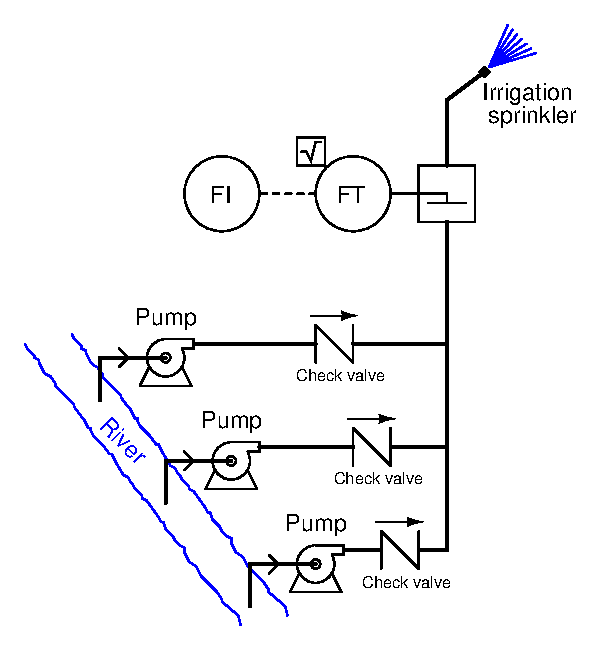
\includegraphics[width=15.5cm]{i01661x01.eps}$$

Tre vannpumper henter vann fra en elv og leverer det til en vanningsspreder. Hva vil skje med vannstrømningsraten over tid hvis en av pumpene slås av (mens de to andre pumpene fortsetter å gå)?

\vskip 10pt

Vil du karakterisere denne prosessen som iboende {\it selvregulerende} eller iboende {\it integrerende}?

\underbar{file i01661no}
%(END_QUESTION)





%(BEGIN_ANSWER)

The water flow rate will very quickly decrease, settling at a new (lower) amount of flow.  This makes it a {\it self-regulating} process.

%(END_ANSWER)





%(BEGIN_NOTES)



%INDEX% Control, process characteristics: self-regulating versus integrating

%(END_NOTES)
